\documentclass[11pt]{IEEEtran}
\usepackage{graphicx}
\usepackage{float}
\usepackage[font=small]{caption}
\title{Getting started with the LOGO! 0BA8 - Setup and I/O configuration}

\author{Gerad Mupfumisi}
\onecolumn
\begin{document}
	\maketitle

\section{Introduction}
\noindent This document presents the process for setting up the LOGO! 0BA8 module for reading and writing to its I/O pins. It also shows how external modules can be linked with the LOGO. The setup will be presented starting at the basic hardware connections required. Examples for reading analogue signals are demonstrated using an analogue voltage source as well as a PT100 temperature sensor. The LOGO! Soft Comfort V8.1 software is used for writing the logic to be performed by the LOGO.  The LOGO! PLC requires a 12V/24V DC source as it's supply. It also requires the LOGO Soft Comfort software for implementing the logic that runs it. On the basic  module, the LOGO has a limited number of digital and analogue inputs. On the outputs, it only has relay contacts that can be used based on the logic running. Digital and analogue inputs/outputs can be added by attaching additional modules. For this report, demonstrations will be made for reading in analogue voltages and temperature values. The AM2 RTD temperature sensor module will be used for reading in the temperature values. This module is used because it has the required circuits that implements the correct signal conditioning for the PT100 temperatures. 

\section{Software Set Up} \label{sec:Software Setup}
\noindent The software side of this demonstration will be run from the LOGO  soft comfort software V8.1. This is an open source software that can be used to program the LOGO in the Functional Block Language or using the Ladder Logic Language. For this demonstration, the Functional Blocks are used. The software can be downloaded from the following website: \textbf{(https://plc4me.com/download-logo-soft-comfort-v8-1-siemens-software-real-100/)}. To install the V8.1 software, first install V7 and then V8.1. The setup files for both versions are available in the zip file downloadable from the link given. Listed below is a step by step instruction set that shows how link the software with the LOGO hardware. After installing the soft comfort software, the first thing to do is connect the logo to the computer via an Ethernet cable and making sure that it can be picked from the software. To do this, launch the software and click on the \textbf{``Network Project"} tab as indicated in Figure\,\ref{fig:network}. Next, click \textbf{``Add New Device"} to open the device selection tab. Select the right device and configuration details. These details can be found on the actual LOGO by following the steps shown in Figure\,\ref{fig:networkDetails}. Click \textbf{``OK"} to finish and the Diagram Editor tab will open automatically. 

\begin{figure}[H]
	\centering
	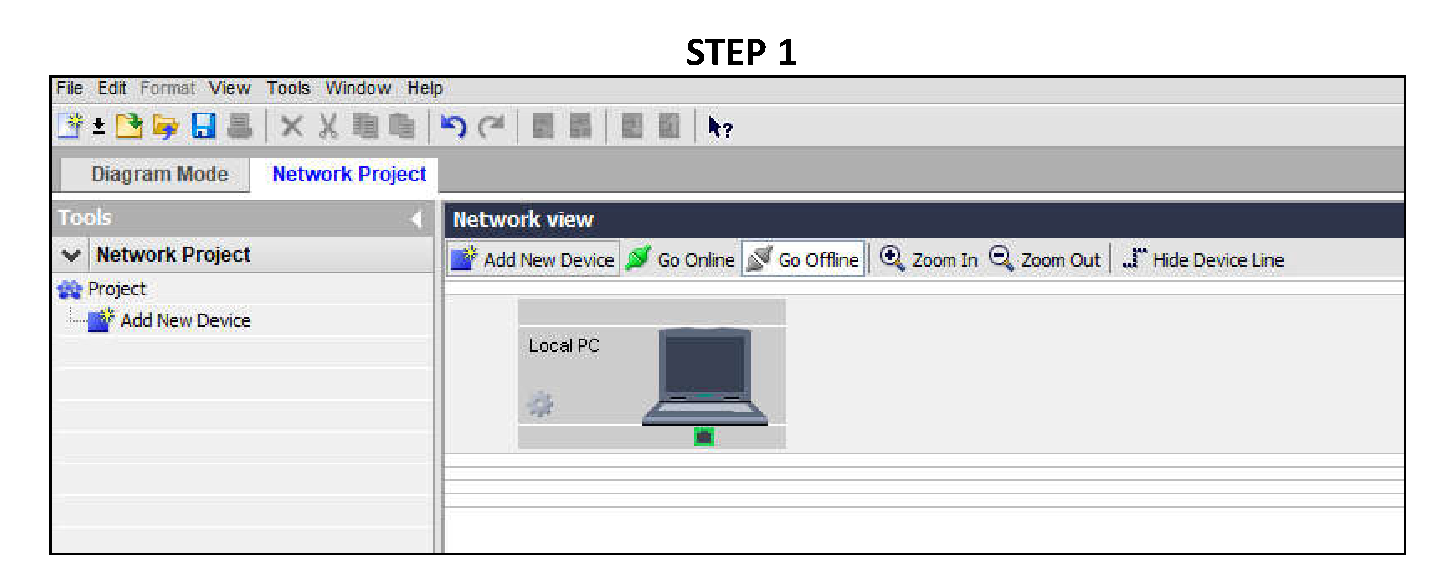
\includegraphics[scale=0.72]{Step1.pdf}
	\caption{Connecting the Logo: Step 1}
	\label{fig:network}
\end{figure}

\begin{figure}[H]
	\centering
	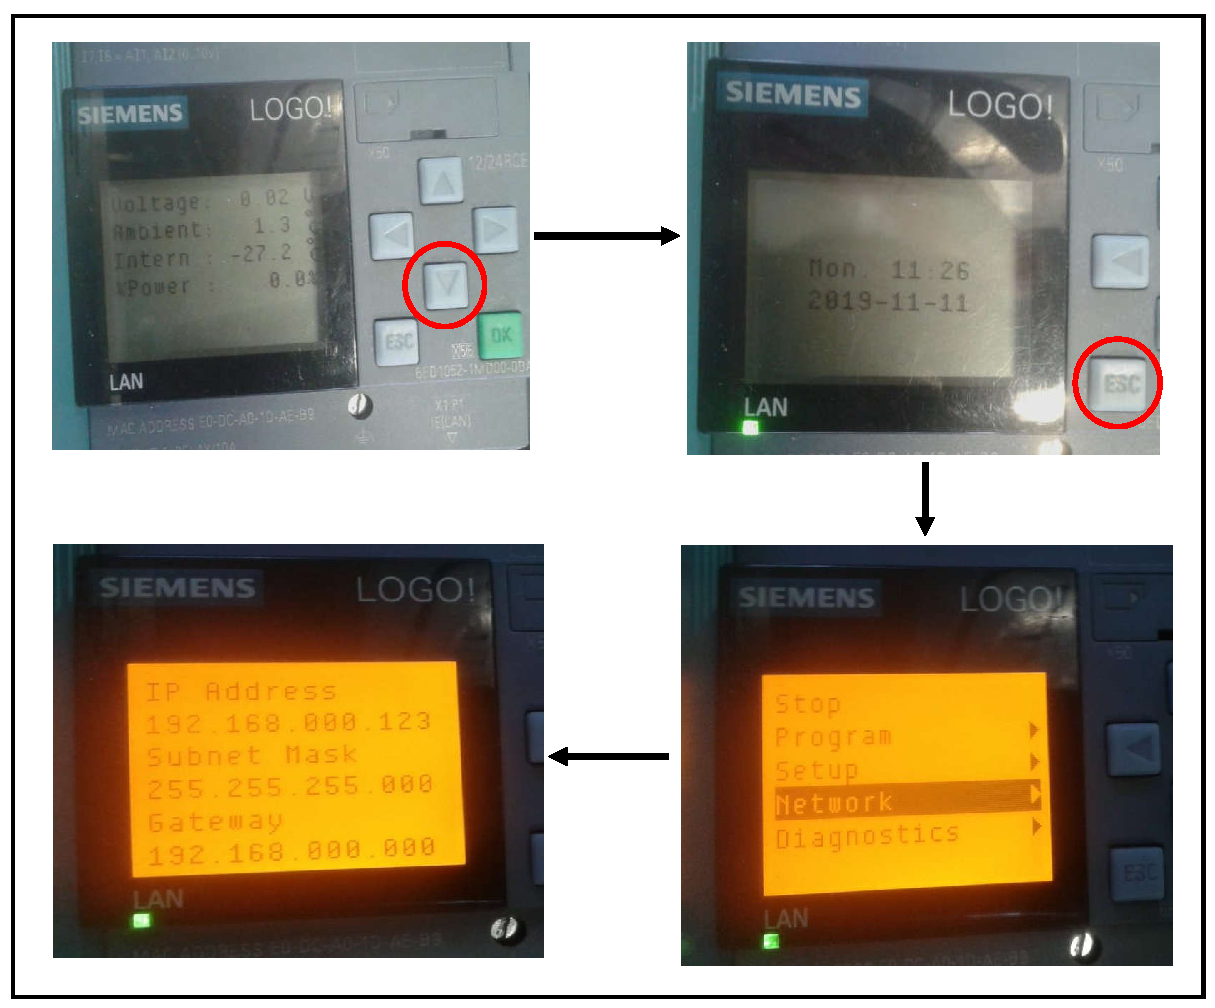
\includegraphics[scale=0.7]{NetworkSettings.pdf}
	\caption{Steps for obtaining the configuration details}
	\label{fig:networkDetails}
\end{figure}
\noindent  Note that there is also a picture which shows that the PC is now connected to a LOGO as shown in Figure\,\ref{fig:ConnectedLogo}. Click the Settings button encircled in the Figure to open the settings Tab. Navigate the I/O Settings and ensure that \textbf{Enable 4 AIs} is selected under \textbf{Onboard AI setting} as shown in Figure\,\ref{fig:Settings}. 

\begin{figure}[H]
	\centering
	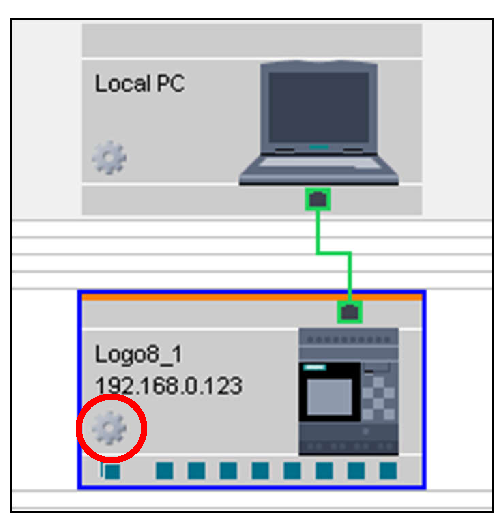
\includegraphics[scale=0.7]{ConnectedLogo.pdf}
	\caption{Logo Connected}
	\label{fig:ConnectedLogo}
\end{figure}

\begin{figure}[H]
	\centering
	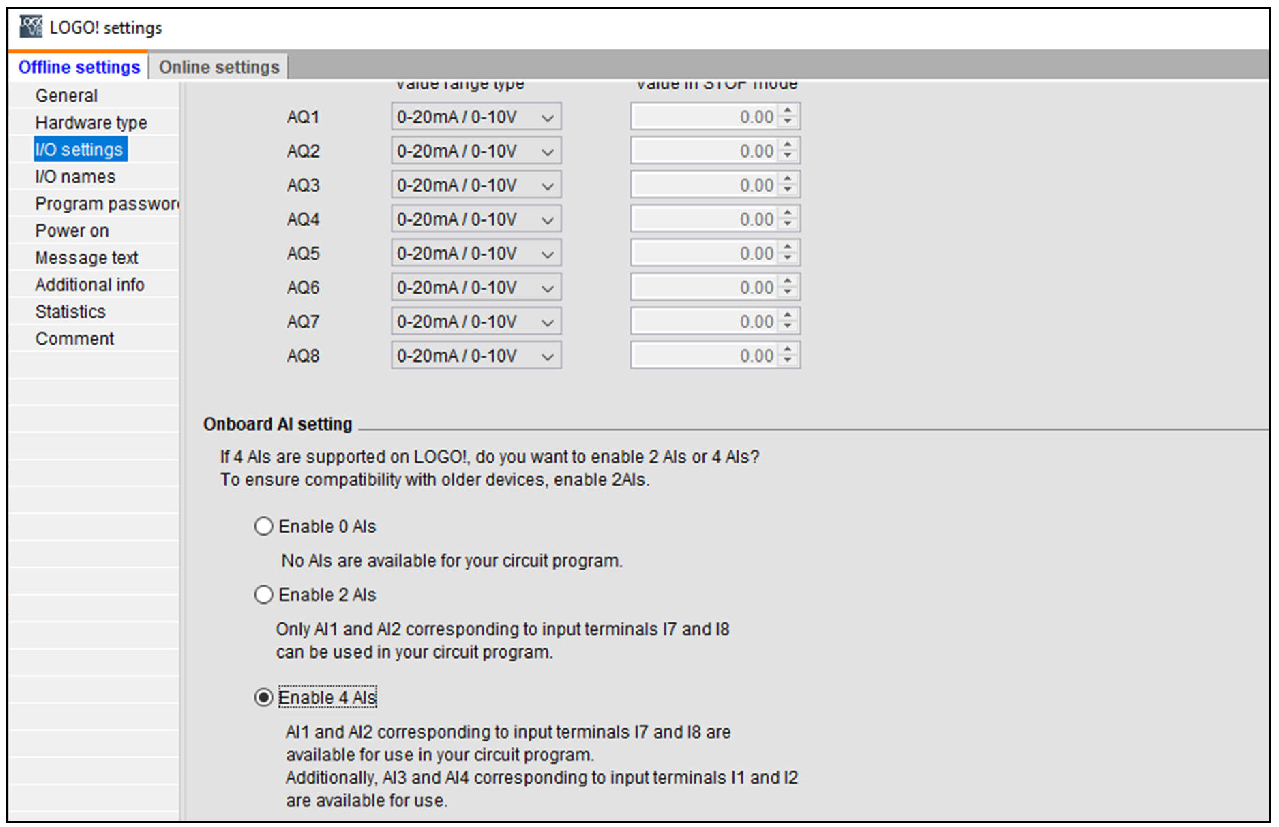
\includegraphics[scale=0.85]{Settings.pdf}
	\caption{Analogue input Settings}
	\label{fig:Settings}
\end{figure}


\noindent In the \textbf{Diagram Editor}, draw the diagram shown in Figure\,\ref{fig:diagram} by dragging and dropping the function blocks from the \textbf{Instructions} drop-down menu located on the left of the screen. In this diagram, \textbf{AI3} represents the analogue input pin that will be used for reading in voltages. This maps to the pin labelled \textbf{I1} on the LOGO. \textbf{AI5} will be for reading in the temperature values. The basic LOGO module only has four analogue input pins. Since the AM2 RTD temperature also reads in analogue values, the LOGO automatically assigns it to to \textbf{AI5}, which is the next available analogue input label. On the actual LOGO, all the input pins are labelled with only \textbf{``I"} on the LOGO which means that all of them can be used as digital inputs. Some pins however are capable of reading both analogue and digital values. Refer to the LOGO manual for more details on the pins and the function blocks. For the correct temperature gain and offset, double click on the Temp Amp block and set the sensor type to PT1000/PT100. Also set the \textbf{Decimal Places} to \textbf{1} for both the Voltage Amp and the Temp Amp. Note that there is a \textbf{Threshold} block connected to analogue input \textbf{AI3} and \textbf{Q1}. \textbf{Q1} is the digital signal that activates the first output relay contacts. The \textbf{Threshold} block will activate the relay when the input goes above the \textbf{on} threshold value and deactivate it when it goes below the \textbf{off} threshold. For this demo, set the upper threshold to 5V and the lower to 4V which correspond to the numbers 400 and 500. This is because the LOGO scales all the input values by 100. To set the messages and variables that will be displayed on the LOGO screen, double click on the \textbf{``Messages"} block. This will open the Messages Tab shown in Figure\,\ref{fig:Messages}. Enter the message to display as shown by step 1. As shown in step 2 and 3, select the variable to be displayed on the LOGO screen. Click the cell to insert the variable and then click Insert Parameter as shown in step 4. Now all the software related work is done, next the hardware configuration is will be done. 

\begin{figure}[H]
	\centering
	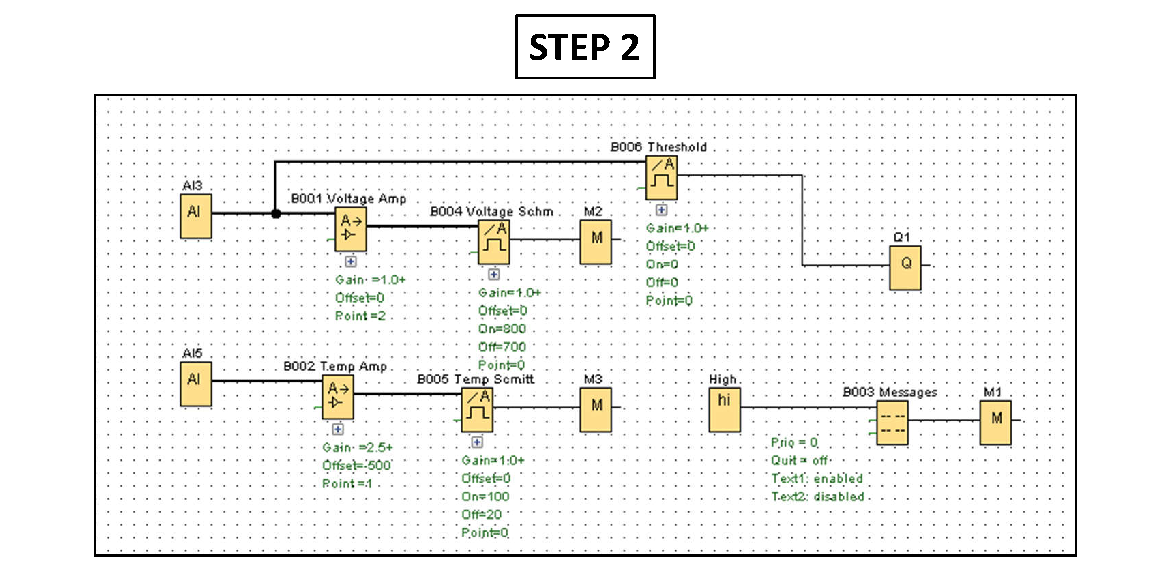
\includegraphics[scale=0.75]{Step2.pdf}
	\caption{Connecting the Logo: Step 2}
	\label{fig:diagram}
\end{figure}

\begin{figure}[H]
	\centering
	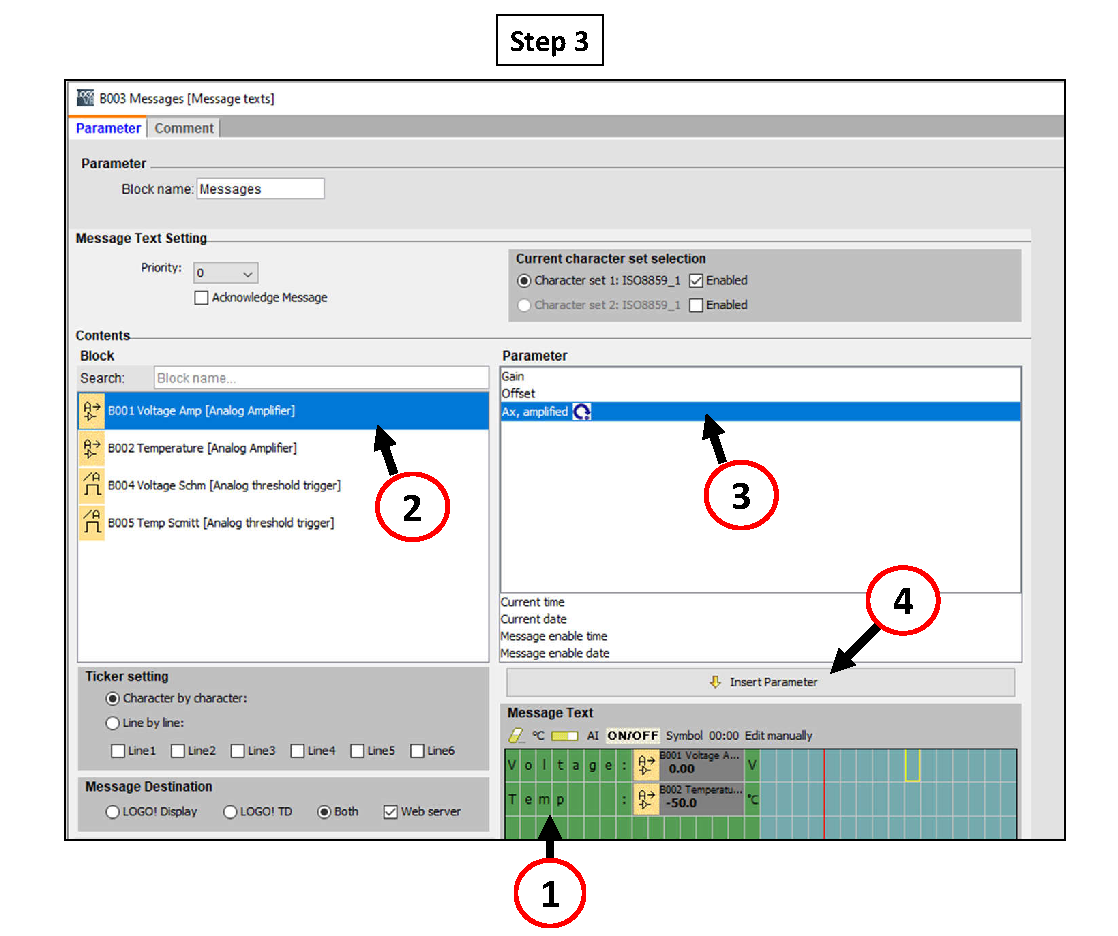
\includegraphics[scale=0.83]{Step3.pdf}
	\caption{Connecting the Logo: Step 3}
	\label{fig:Messages}
\end{figure}

\section{Basic Hardware Setup}
\noindent Figure\,\ref{fig:basic wiring} shows how the LOGO should be wired for this demonstration. 
\begin{figure}[H]
	\centering
	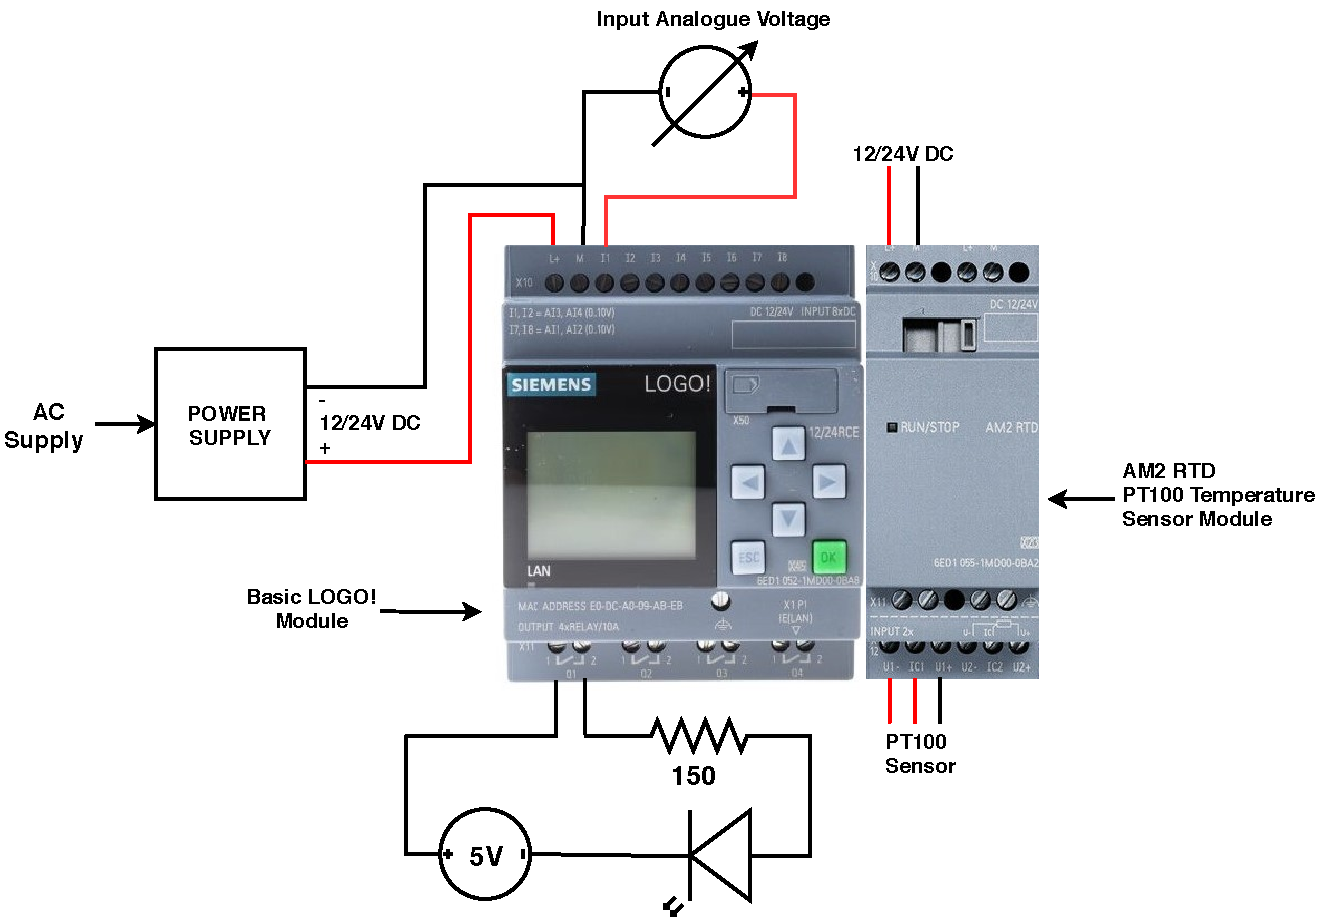
\includegraphics[scale=0.6]{LogoBasicWiring.pdf}
	\caption{Basic wiring of the LOGO}
	\label{fig:basic wiring}
\end{figure}

\section{Upload the program into the LOGO}
\noindent To upload the program into the LOGO, click the button \textbf{``PC to LOGO"} as shown in Figure\,\ref{fig:PCtoLOGO}. This will open the Interface shown in Figure\,\ref{fig:PCtoLOGO2}. Click the refresh button in step 1 to locate all the LOGO modules connected to the PC. Once located, the details of the LOGO will appear as shown. Ensure that these details match with those entered in Section\,\ref{sec:Software Setup}. Click on the the LOGO as shown in step 2. Click the \textbf{Test} button to verify that the PC can communicate with LOGO. After a green confirmation tick appears, click \textbf{OK} and agree (Click Yes) to all the pop up prompts that will follow. This will upload the program in into the LOGO. 
\begin{figure}[H]
	\centering
	
\includegraphics[scale=0.8]{PCtoLOGO.pdf}
	\caption{PC to LOGO Button}
	\label{fig:PCtoLOGO}
\end{figure}

\begin{figure}[H]
	\centering
	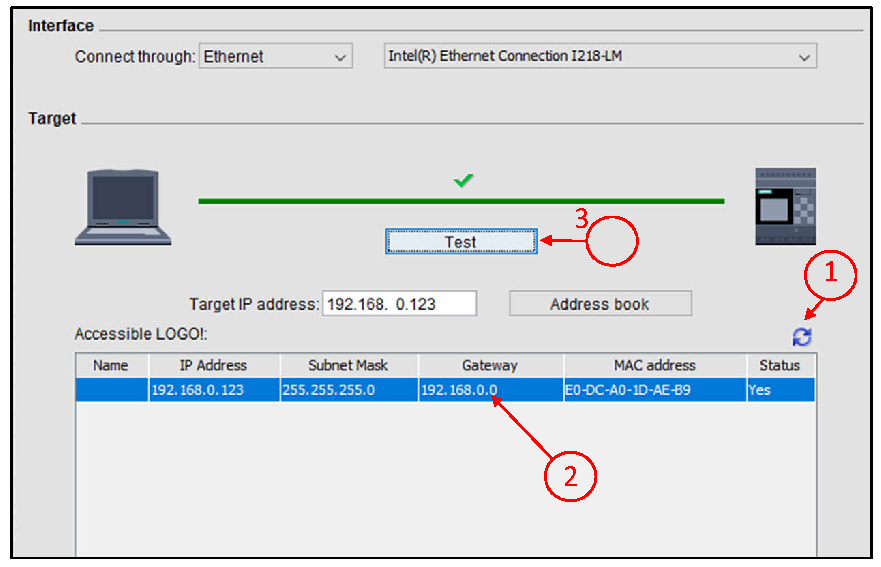
\includegraphics[scale=0.6]{PCtoLOGO2.pdf}
	\caption{Select the LOGO}
	\label{fig:PCtoLOGO2}
\end{figure}

\section{Test the LOGO}
\noindent There are three things that will be tested. First is the analogue reading of the input voltage. Vary the supply voltage and observe the readings shown on the screen of the LOGO. Next observation will be to test the relay output. Increase the variable input voltage until it goes above 5V. Notice that when it goes above this value, the output LED switches on. Now decrease the voltage. Notice that the LED only turns off after the voltage drops to below 4V. Finally, test the temperature sensor. Expose the tip of the PT100 sensor to different temperatures and observe the temperature reading shown on the screen of the LOGO. In this demo, the tip was placed in a refrigerator which is expected to maintain a temperature around 7$^o$C. Figure\,\ref{fig:testing} shows a picture of the LOGO running the program and giving the results as explained above. 

\begin{figure}[H]
	\centering
	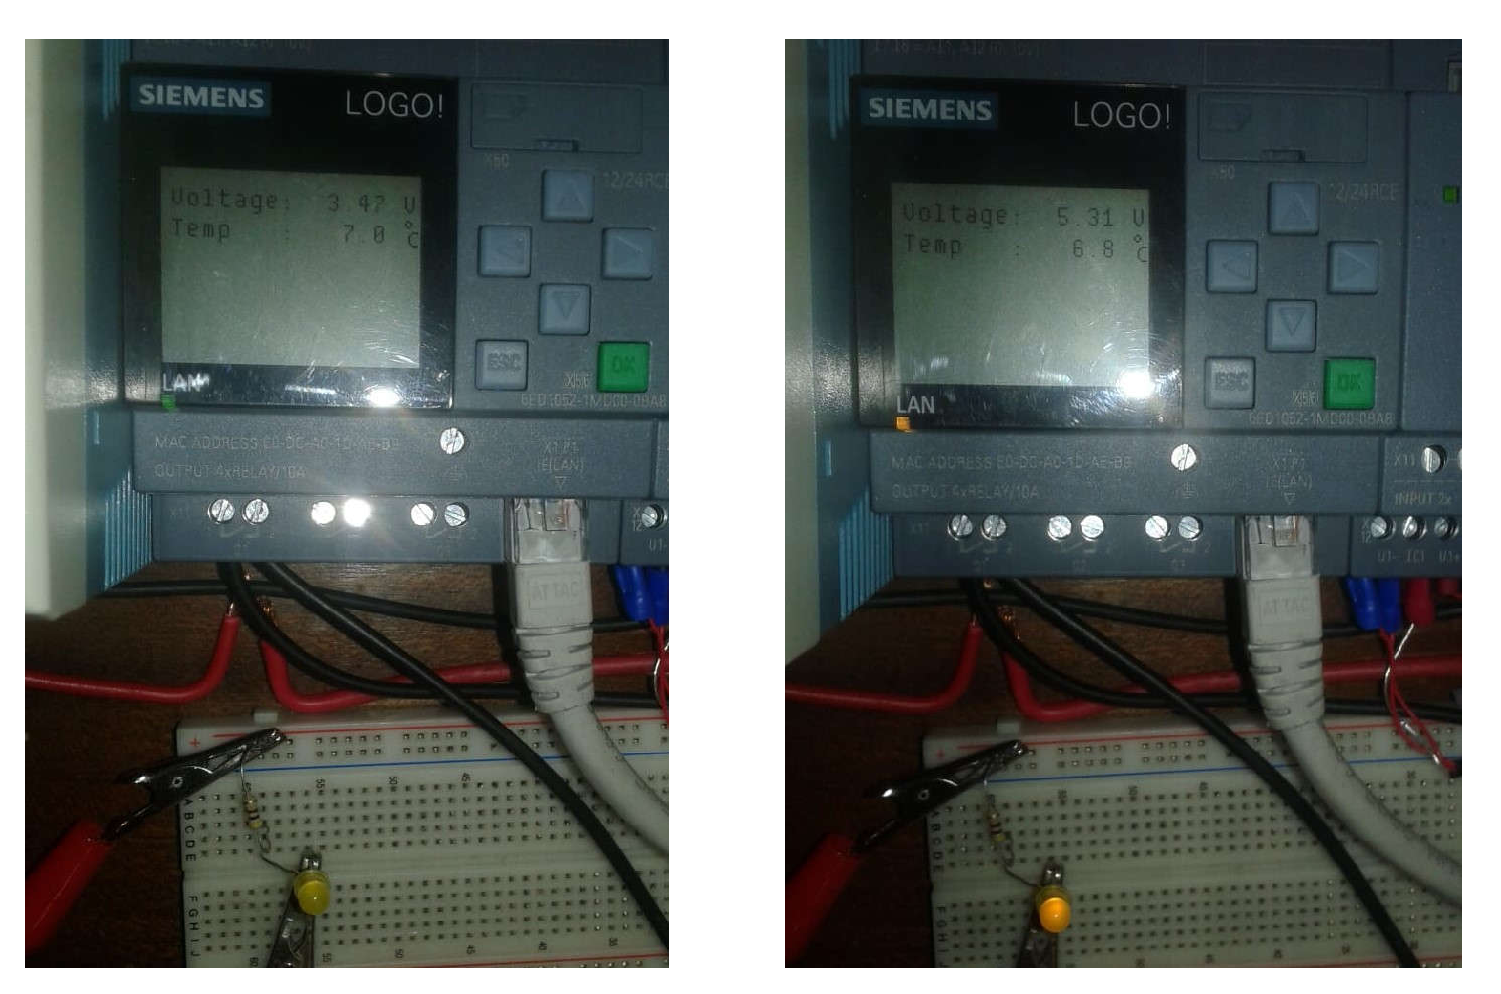
\includegraphics[scale=0.6]{Result.pdf}
	\caption{Testing the LOGO}
	\label{fig:testing}
\end{figure}


\section{Conclusion}
\noindent This document gave the basic instructions needed for getting started with using the LOGO PLC module. The software needed to run was discussed and the setup process was given. A basic hardware wiring diagram was presented to show how to physically connect the LOGO. Some basic results were presented to demonstrate the basic operation of the LOGO.
 

\end{document}